This layer is the actual shutter which takes requests and tries to complete the task, if the task is successfully completed it send an acknowledgement. This layer has two subsystems which are the motor commands and acknowledge completed inputs

\begin{figure}[h!]
	\centering
 	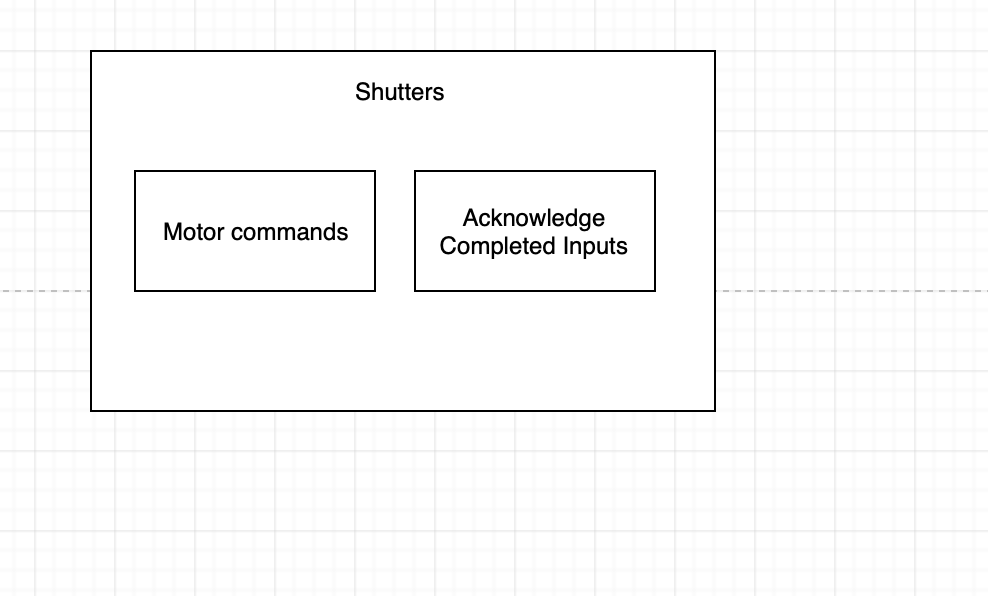
\includegraphics[width=0.60\textwidth]{images/Shutters}
 \caption{Example subsystem description diagram}
\end{figure}

\subsection{Motor Commands}
This subsystem is responsible for taking requests sent from the hub and completing the task.

\subsubsection{Assumptions}
Users have an android or ios phone and users have not tampered with the hub and shutters.

\subsubsection{Responsibilities}
This subsystem should be able to take request from the hub and complete them with no issues

\subsubsection{Subsystem Interfaces}


\begin {table}[H]
\caption {Subsystem interfaces} 
\begin{center}
    \begin{tabular}{ | p{1cm} | p{7cm} | p{5cm} | p{3cm} |}
    \hline
    ID & Description & Inputs & Outputs \\ \hline
    1 & Package all request and send to the shutters & Bluetooth communication & Motor commands\\ \hline
    \end{tabular}
\end{center}
\end{table}

\subsection{Acknowledge Completed Inputs}
This subsystem is responsible for sending acknowledgements to the mobile application upon task completion.

\subsubsection{Assumptions}
Users have an android or ios phone and users have not tampered with the hub and shutters.

\subsubsection{Responsibilities}
This subsystem should be able to send acknowledgements to the mobile application upon task completion

\subsubsection{Subsystem Interfaces}

\begin {table}[H]
\caption {Subsystem interfaces} 
\begin{center}
    \begin{tabular}{ | p{1cm} | p{7cm} | p{5cm} | p{5cm} |}
    \hline
    ID & Description & Inputs & Outputs \\ \hline
    1 & Send an acknowledgement on task completion & Acknowledge completed inputs & Mobile Application\\ \hline
    \end{tabular}
\end{center}
\end{table}
